\documentclass[
  scale = 1.5,
  advisor = {{https://github.com/nachos-con-queso/HFT-Poster}},
  authorLabel = {{(jens@calov.net)}},
  advisorLabel = {{(Download-URL)}},
]{hftpostr}

\title{Thesis-Poster mit \LaTeX}
\author{Jens Calov}

\usetheme{PosterHFT1}

\usepackage{qrcode}


\begin{document}

\begin{frame}[fragile, t]

  \begin{block}{Motivation}
    Wenn man an der HFT Stuttgart im Studienbereich Mathematik eine Bachelor- oder Master-Thesis schreibt, so gehört auch die Erstellung eines Posters dazu.
    Hierfür stellt die Hochschule eine Microsoft PowerPoint-Vorlage zur Verfügung, die bislang zwingend zu verwenden ist.
    Gerade im Bereich Mathematik ist \LaTeX\ jedoch das Standard-Werkzeug schlechthin.
    Es sollte allen Studierenden ermöglicht werden, nicht nur die Abschlussarbeit mit \LaTeX\ zu schreiben, sondern auch das entsprechende Plakat mit \LaTeX\ zu erstellen.
    Zudem sollte auch grundsätzlich der OpenSource-Gedanke gefördert werden und die Abhängigkeit von proprietärer Software verringert werden.
    Deshalb wurde nun eine \LaTeX-Dokumentenklasse entwickelt, die die PowerPoint-Vorlage ersetzen kann.
  \end{block}

  \vskip-2ex

  \begin{columns}[onlytextwidth, T]
      \begin{column}{.31\textwidth}
        \begin{block}{Genutzte Technologie}
          Im Wesentlichen nutzt die neue \LaTeX-Dokumentenklasse das über CTAN verfügbare Package \textit{beamerposter}, das eine Erweiterung der Klassen \textit{beamer} und \textit{a0poster} ist.
          Darauf aufbauend werden in der neuen Dokumentenklasse \textit{hftpostr} einige Einstellungen vorgenommen, die das Design der HFT-Vorlage nachahmen.
          Die weiteren \textit{Beamer-Themes} \textit{PosterHFT1} und \textit{PosterHFT2} bieten Möglichkeiten, das Design des Posters einfach zu ändern.
        \end{block}
      \end{column}
      \begin{column}{.31\textwidth}
        \begin{block}{Dateien}
          Die folgenden Dateien werden mit der Vorlage geliefert und sind zur Nutzung aller Funktionen notwendig:
          \begin{itemize}
            \item \texttt{beamerthemePosterHFT1.sty}
            \item \texttt{beamerthemePosterHFT2.sty}
            \item \texttt{hftpostr.cls}
            \item \texttt{hftpostrbackground.pdf}
          \end{itemize}
          Das vorliegende Poster wurde mit diesen Dateien erzeugt:
          \begin{itemize}
            \item \texttt{example.tex}
            \item \texttt{exampleFigure.pdf}
          \end{itemize}
        \end{block}
      \end{column}
      \begin{column}{.31\textwidth}
        \begin{block}{Kollaboration}
          Falls Du Fehler findest, Verbesserungsvorschläge oder einfach nur eine Idee dazu hast:
          \begin{center}
            \vskip-1.5ex
            \textcolor{HFTred1}{\textbf{Bitte melde Dich!}}
          \end{center}
          Die Vorlage kann nur besser werden, wenn Du auch sagst was Dich stört oder was Du Dir wünschst.
          Wer einen GitHub-Account hat, kann auch direkt auf der Projektseite (URL s.u.) ein Issue erstellen.
          Wer \LaTeX-begeistert ist, darf gerne direkt an der Verbesserung der Vorlage mitwirken!
        \end{block}
      \end{column}
  \end{columns}

  \vskip1ex

  \begin{columns}[onlytextwidth, T]
      \begin{column}{.75\textwidth}
        \begin{block}{Verwendung}
          In der Datei \texttt{main.tex} werden die Inhalte des Posters hauptsächlich mit zwei Umgebungen gesetzt: \textit{block} und \textit{columns}.
          Hier ein Beispiel:

          \begin{columns}[onlytextwidth, T]
            \begin{column}{.4\textwidth}
              \begin{lstlisting}[
                  basicstyle=\footnotesize, %or \small or \footnotesize etc.
              ]
  \begin{columns}[onlytextwidth, T]
  \begin{column}{.48\textwidth}
    \begin{block}{Blocktitel links}
      Hier steht der Inhalt eines linken Blocks.
    \end{block}
  \end{column}
              \end{lstlisting}
            \end{column}
              \vrule{}
            \begin{column}{.51\textwidth}
              \begin{lstlisting}[
                  basicstyle=\footnotesize, %or \small or \footnotesize etc.
              ]
    \begin{column}{.48\textwidth}
      \begin{block}{Blocktitel rechts}
        Hier steht der Inhalt eines rechten Blocks.
      \end{block}
    \end{column}
  \end{columns}
              \end{lstlisting}
            \end{column}
          \end{columns}
          \vspace{1em}
          Zudem stehen die drei Themes \textit{default}, \textit{PosterHFT1} und \textit{PosterHFT2} zur Verfügung.
          Die Auswahl erfolgt über den Befehl \texttt{\textbackslash usetheme\{\}}.
           Das hier dargestellte Poster verwendet das Theme \textit{PosterHFT1}.
        \end{block}
      \end{column}
      \begin{column}{.21\textwidth}
        \begin{block}{Link zum Download der Dokumentenklasse}
        \qrcode[hyperlink, height=10.5cm]{https://github.com/nachos-con-queso/HFT-Poster/}
        \end{block}
      \end{column}
  \end{columns}


  \begin{block}{Beispiel für Mathematik-Umgebung: Faltung als Schichtübergang in einem Feedforward-Netz}

    \begin{columns}[onlytextwidth, T]
      \begin{column}{0.31\textwidth}
      \begin{itemize}
          \item Faltung (eigentlich Kreuzkorrelation):
            \[
             \begin{pmatrix}
               a & b & c\\
               d & e & f\\
               g & h & i
             \end{pmatrix}
             *
             \begin{pmatrix}
               \textcolor{ForestGreen}{\alpha} & \textcolor{Blue}{\beta}\\
               \textcolor{BrickRed}{\gamma} & \textcolor{Dandelion}{\delta}
             \end{pmatrix}
             =
             \begin{pmatrix}
               w & x\\
               y & z
             \end{pmatrix}
            \]
        % \vspace{-.5em}
          \item Feedforward-Netz-Schichten:
            \begin{align*}
              U_i &=  \{ v_a, v_b, v_c, v_d, v_e, v_f, v_g, v_h, v_i \}\\
              U_{i+1} &= \{ u_w, u_x, u_y, u_z \}
            \end{align*}
          % \vspace{-1.5em}
          \item Gewichtsmatrix:
            \begin{align*}
              W_{U_{i+1}} =
              \begin{pmatrix}
                \textcolor{ForestGreen}{\alpha} & \textcolor{Blue}{\beta} & 0 & \textcolor{BrickRed}{\gamma} & \textcolor{Dandelion}{\delta} & 0 & 0 & 0 & 0\\
                0 & \textcolor{ForestGreen}{\alpha} & \textcolor{Blue}{\beta} & 0 & \textcolor{BrickRed}{\gamma} & \textcolor{Dandelion}{\delta} & 0 & 0 & 0\\
                0 & 0 & 0 & \textcolor{ForestGreen}{\alpha} & \textcolor{Blue}{\beta} & 0 & \textcolor{BrickRed}{\gamma} & \textcolor{Dandelion}{\delta} & 0\\
                0 & 0 & 0 & 0 & \textcolor{ForestGreen}{\alpha} & \textcolor{Blue}{\beta} & 0 & \textcolor{BrickRed}{\gamma} & \textcolor{Dandelion}{\delta}\\
              \end{pmatrix}
            \end{align*}
        \end{itemize}
      \end{column}
      \begin{column}{0.42\textwidth}
    	\begin{itemize}
    		\item Netzeingabe der Schicht ${U_{i+1}}:$
    	\end{itemize}
    \begin{align*}
    		net_{U_{i+1}} &=	W_{U_{i+1}} \, out_{U_i}\\
        &=
    		\begin{pmatrix}
    			\textcolor{ForestGreen}{\alpha} & \textcolor{Blue}{\beta} & 0 & \textcolor{BrickRed}{\gamma} & \textcolor{Dandelion}{\delta} & 0 & 0 & 0 & 0\\
    			0 & \textcolor{ForestGreen}{\alpha} & \textcolor{Blue}{\beta} & 0 & \textcolor{BrickRed}{\gamma} & \textcolor{Dandelion}{\delta} & 0 & 0 & 0\\
    			0 & 0 & 0 & \textcolor{ForestGreen}{\alpha} & \textcolor{Blue}{\beta} & 0 & \textcolor{BrickRed}{\gamma} & \textcolor{Dandelion}{\delta} & 0\\
    			0 & 0 & 0 & 0 & \textcolor{ForestGreen}{\alpha} & \textcolor{Blue}{\beta} & 0 & \textcolor{BrickRed}{\gamma} & \textcolor{Dandelion}{\delta}\\
    		\end{pmatrix}
    		\,
    		\begin{pmatrix}
    			a\\
    			b\\
    			c\\
    			d\\
    			e\\
    			f\\
    			g\\
    			h\\
    			i
    		\end{pmatrix}
    		=
    		\begin{pmatrix}
    			w\\
    			x\\
    			y\\
    			z\\
    		\end{pmatrix}
    \end{align*}
      \end{column}
      \begin{column}{0.23\textwidth}
        \begin{center}
          \begin{figure}
            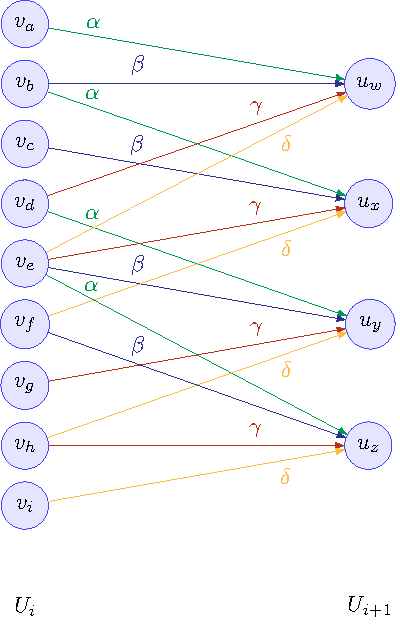
\includegraphics[width=.8\textwidth]{exampleFigure.pdf}
          \end{figure}
        \end{center}
      \end{column}
    \end{columns}

  \end{block}



\end{frame}

\end{document}
